% !TeX root = ../../Thesis.tex
\chapter{Introduction}
\label{chp:introduction}
The material presented in this thesis represents kinetic simulations of laser-plasma interactions (\acrshort{LPI}) relevant to direct-drive inertial confinement fusion (\acrshort{ICF}). In this introductory chapter, an overview of the goals of, and approaches to, inertial confinement fusion is given; including specific details of the `shock-ignition' (\acrshort{SI}) ICF scheme. We then review the previous work concerning laser-plasma interactions in direct-drive ICF, and motivate the use of kinetic modelling throughout this thesis. Finally, we offer an outline of the rest of the thesis.

\section{Inertial Confinement Fusion}
The basic concept of inertial confinement fusion (\acrshort{ICF}) is based on the Ulam-Teller design for a thermonuclear weapon (H-bomb), which uses radiation to compress thermonuclear fuel to the point where it undergoes nuclear fusion \citep{SpanishHistoryOfICF}.  Nuclear fusion is the process by which two light atomic nuclei overcome to electric repulsion between them and combine to form a new, heavier, nucleus and release energy proportional to the mass gap as kinetic energy of the fusion products. The reaction of choice in the thermonuclear weapon, and in most modern ICF designs, is deuterium-tritium (\acrshort{DT}) fusion. Equation \ref{eq:DTfusion} shows the \acrshort{DT}  reaction; first in the most commonly-presented formula, and then explicitly in terms of the ions and their neutron (superscript) and proton (subscript) numbers.

\begin{equation}\label{eq:DTfusion}
\begin{aligned}
	\text{D} + \text{T} &\longrightarrow \text{He}^4 + \text{n} + 17.6 \si{\mega\electronvolt}\\
	{}^2_1\text{H} + {}^3_1\text{H} &\longrightarrow {}^4_2\text{He} (3.5\si{\mega\electronvolt}) + {}^1_0\text{n} (14.1\si{\mega\electronvolt}).
\end{aligned}
\end{equation}
In order for a fusion reaction to be usable on earth, we require that it satisfies certain criteria: uses the lightest possible elements; reaction occurs at `reasonable' temperatures (on the order of $10 \si{\kilo\eV}$); reactants (fuel) are obtainable. Figure \ref{fig:crossSection} shows that the \acrshort{DT} reaction has the largest cross section / highest thermal reactivity of the several reactions which satisfy the above conditions.

\begin{figure}
 \centering
 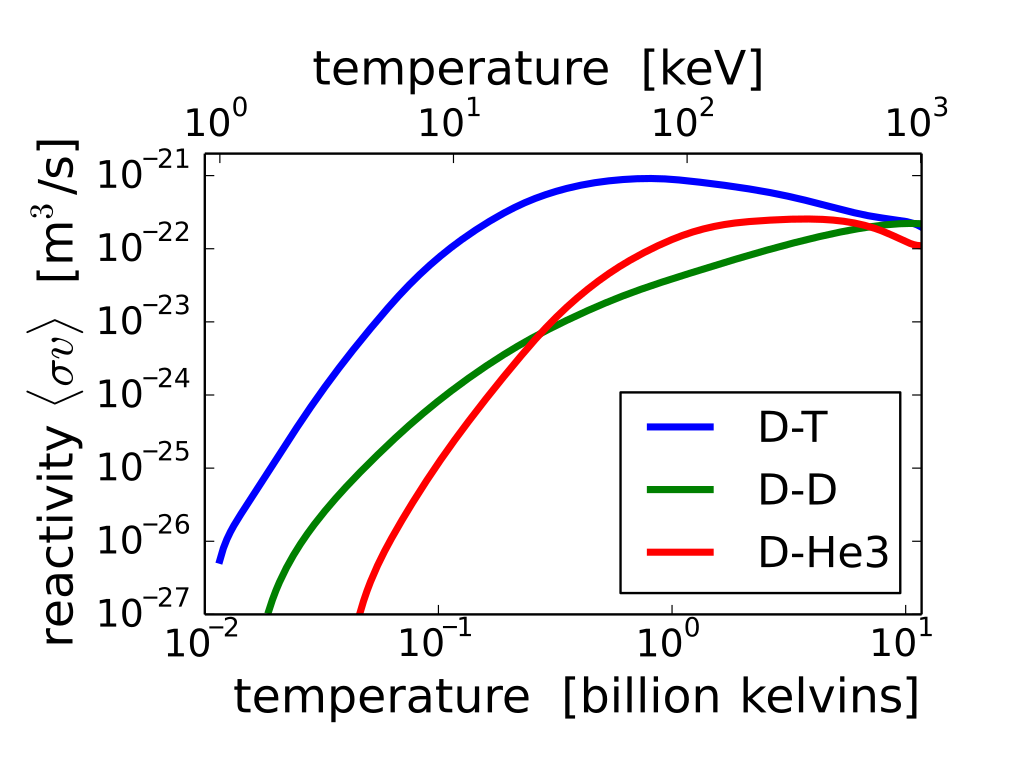
\includegraphics[width=0.7\columnwidth]{Chapters/C1_Introduction/crossSection.png}
 \caption{Thermal reactivity (product of interaction cross-section and velocity averaged over a Maxwellian) as a function of temperature: for deuterium-tritium, deuterium-deuterium (both interaction branches), and deuterium-helium nuclear reactions. Re-printed from \url{https://commons.wikimedia.org/wiki/File:Fusion_rxnrate.svg} under a Creative Commons 2.5 license, via Wikimedia Commons.} \label{fig:crossSection}
\end{figure}

In a thermonuclear weapon the radiation source is a fission bomb (also known as an `atom bomb' or `A-bomb'), which detonates and reaches very high temperatures, producing thermal x-rays which are channelled to compress the thermonuclear fuel. The fusion reaction which results from the high density and temperature conditions created in the compressed fuel is unconfined and, therefore, unsuited for energy generation. When lasers were proposed and realised, by \citet{Maser1958} and \citet{Maiman1960} respectively, scientists at Lawrence Livermore National Laboratory realised that lasers had the potential to ignite fusion explosions without using an atomic bomb. In 1972, \citet{Nuckolls1972} published a paper in Nature in which they used the LASNIX computer code to show that high-energy lasers could be used to compress hydrogen to super-high densities. Combined with small target pellets of fusion fuel, which will undergo burn before exploding (due to their inertia), the basic idea of inertial-confinement fusion (\acrshort{ICF}) was born. We now know that \acrshort{ICF} was demonstrated successfully in underground nuclear tests, just ten years after Nuckolls proposed it, but with a fission bomb as the driver, rather than a laser \citep{Evans2010}.




\subsection{Direct and indirect drive ICF}
Developments on the basic ICF scheme can be categorised by how the laser is used to perform the radiation compression of the fuel. In laser indirect-drive (\acrshort{LID}) models, fusion fuel is held inside a hollow chamber made of a high atomic number material. This structure is known as the hohlraum, from the German for `hollow space'. Lasers are then used to heat the inside walls of the hohlraum until they emit a bath of X-rays which heat the outer layer of the fuel capsule, causing the outer layer of the capsule to ablate and a rocket-effect-like implosion of the inner fuel. It is clear that this process is very similar to the indirect approach used to drive the thermonuclear explosion in the Ulam-Teller design. As such, the National Ignition Facility (\acrshort{NIF}) (US) and Laser M\'{e}gajoule (\acrshort{LMJ}) (France) are set-up for indirect-drive ICF, in order to support their respective country's nuclear weapons research programmes. An advantage of the indirect-drive technique is that the absorption and re-emission of laser energy by the hohlraum smooths the radiation which will drive the implosion.

Improvements in laser smoothing technology have made this advantage of \acrshort{LID} less obvious, and much research now focuses on laser direct-drive (\acrshort{LDD}). In laser direct-drive the laser beams are aimed at the target directly. Go through the steps: ablation; shocks; shocks; ignition. One limit to the success of any direct-drive scheme is the direct interaction of the laser with the coronal plasma. 





\subsection{Shock-ignition}
 This is a directly-driven central ignition scheme boosted by a strong shock.

\begin{figure}
 \centering
 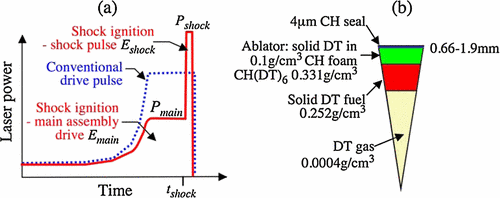
\includegraphics[width=0.8\columnwidth]{Chapters/C1_Introduction/SI_profile.png}
 \caption{Shock-ignition design for the National Ingition Facility (NIF) Reprinted with permission from \citep{Perkins2009}. (all licenses are in Appendices)} \label{fig:SI_laser}
\end{figure}


\section{Previous work}
\subsection{Laser-plasma interactions in shock-ignition}

Incident laser radiation drives a collective wave in a plasma to high amplitude, this wave then scatters in incident laser such that the beating of the laser and the scattered light ponderomotively drives electrons into bunches with a wavelength matching the initial plasma wave.

\subsection{Simulations}
\subsubsection{Kinetic models}
\subsubsection{Fluid models with kinetic effects}
Basically it's interesting that you can put some of these effects into a fluid model, such as here \citep{Tran2020}
\subsection{Experiments}

\subsection{Why PIC in this thesis?}
Question: doesn't PIC suck for predicting experimental observables? 

Need kinetics. Too expensive to use VFP for these laser-plasma interactions since the WFP velocity grid must be fine enough to resolve the electron quiver velocity. Also we have a PIC code in-house.

\section{Thesis Outline}
In the next five chapters, the wokr h uhuihuh uhi 

\begin{description}
	\item[Chapter 2] We present in Chapter \ref{chp:theory} the theory of laser-plasma interactions relevant to this thesis. We derive,... blah is introduced ... We describe the basic linear, quasi-linear, and non-linear theory required to understand normal modes; wave-particle interactions; and wave-wave instabilities, respectively, which are relevant to the coronal plasmas in direct-drive ICF.
	
	\item[Chapter 3] Here we present the EPOCH particle-in-cell (\acrshort{PIC}) code, which is used to perform all the simulations presented in this thesis, alongside a review of the PIC method for kinetic plasma simulations. Basic benchmarking of the code to the theory presented in Chapter \ref{chp:theory} is performed, and we introduce several key diagnostics which are used throughout the thesis.
	 
	\item[Chapter 4] In this work, we use one-dimensional particle-in-cell 		
		simulations to show that there is a non-linear frequency shift caused  
		by kinetic effects, resulting in the growth of SRS in an inhomogeneous 
		plasma far exceeding the predictions of fluid theory, so-called 
		inflationary SRS or iSRS. We find that iSRS occurs over a wide range of 
		density scale-lengths relevant to shock-ignition and other directly-
		driven inertial confinement fusion schemes. Here we quantify the 
		intensity threshold for the onset of iSRS for shock-ignition relevant 
		parameters.
	\item[Chapter 5] In this chapter, results of one-dimensional PIC simulations are presented, which represent the first investigation into the practical possibility of using broadband to suppress inflationary SRS in shock-ignition. We show that for a decoupled broadband laser, the non-linear frequency shift must be taken into account when calculating the condition for suppression of iSRS. Next we consider the case of realistic shock-ignition schemes on three laser systems: frequency-tripled Nd : glass; Krypton Fluoride (KrF); and Argon Fluoride (ArF).
	\item[Chapter 6] Here we present 
\end{description}

\section*{Conventions adopted in the thesis}
Unless otherwise stated in the text, all equations and physical quantities in this thesis are in SI units. Standard SI prefixes (k for kilo, T for tera- etc) are used. All numerically-calculated values are given to two significant figures, and written in scientific notation for values greater than 1000, and less than $1/1000$.

%\bibliographystyle{plainnat}
%\bibliography{Chapters/C1_Introduction/Introduction}
